\chapter{Trabajo relacionado y Estado del Arte} \label{chp:state-of-the-art}

En este capítulo se cubre el estado del arte de la energía solar fotovoltaica y, particularmente, de la librería \textit{pvlib-python}. Se podrá encontrar en las siguientes secciones:

\begin{itemize}

      \item[•] \fullref{sct:energia-solar}: explica el estado actual de la energía solar fotovoltaica y su fundamento teórico base.

      \item[•] \fullref{sct:simulaciones}: detalla las herramientas de simulación utilizadas en el sector fotovoltaico y el marco general de comparación de la librería \textit{pvlib-python}.

      \item[•] \fullref{sct:pvlib}: presenta las características de la biblioteca \textit{pvlib-python}.

\end{itemize}

%%%%%%%%%%%%%%%%%%%%%%%%%%%%%%%%%%%%%%%%%%%%%%%%%%%%%%%%%%%%%%%%%%%%%%%%%%%%%%%%
%%%%%%%%%%%%%%%%%%%%%%%%%%%%%%%%%%%%%%%%%%%%%%%%%%%%%%%%%%%%%%%%%%%%%%%%%%%%%%%%

\section{La energía solar fotovoltaica} \label{sct:energia-solar}

En esta sección se presentará el estado del arte de las diferentes tecnologías, estudios y sistemas relacionados con la energía solar fotovoltaica.

La energía solar fotovoltaica es una tecnología que convierte la radiación solar en electricidad utilizando células solares mediante el efecto fotoeléctrico \cite[][pp. 701-706]{böer2002survey}.
Este fenómeno consiste en la generación de una corriente eléctrica cuando la luz incide sobre un material semiconductor y excita los electrones de la banda de valencia a la banda de conducción. Esta excitación genera un par electrón-hueco que se separa por la acción de un campo eléctrico externo (en cuyo caso no se produce energía neta positiva) o mediante la distribución de cargas en un semiconductor p-n, que permite la extracción de energía. Este último caso es el de aplicación en células solares fotovoltaicas, pues la intención es obtener energía eléctrica.

Existen varias tecnologías de células solares, como las de silicio, las de película delgada y, las más experimentales, de concentración y de otros materiales orgánicos y multiunión, que se agrupan en generaciones \cite{Shubbak_2019}. Cada generación responde a una serie de características e implantación en el mercado, donde destacan:

\begin{itemize}
      \item Primera generación: células de silicio monocristalino y policristalino.
            Se encuentran bien implantadas en el mercado y son las más utilizadas en aplicaciones fotovoltaicas. Según el límite teórico que calcularon Shockley y Queisser en 1961, el silicio es el material más apropiado para la fabricación de células solares, ya que su banda prohibida de $1.1 eV$ es la que mejor se ajusta al máximo de la radiación solar \cite[][p. 1126]{böer2002survey}. Sin embargo, presentan un coste de producción moderado y un alto uso de material. El límite de eficiencia teórico obtenido por los anteriores autores es del 33.7\% \cite{Shockley_Queisser_1961} para colectores planos y células solares de una sola unión, es decir, que no tratan ni con sistemas de concentración ni células multiunión o tándem.
      \item Segunda generación: células de película delgada, como las de telururo de cadmio ($CdTe$), las de di-seleniuro de cobre, indio y galio (\textit{Copper indium gallium selenide}, $CuInGaSe_2$), las de arseniuro de galio (\textit{Gallium arsenide}) ($GaAs$) y las de silicio amorfo ($\text{a-Si:H}$).
            Destacan por ser de capa delgada (\textit{thin-film}) y, consecuentemente, más baratas de producir por el bajo uso de material, si bien pueden llegar a ser composiciones de materiales más caros.
            Nótese que el silicio amorfo es ampliamente utilizado, en especial en aplicaciones de baja potencia, como calculadoras, pero su eficiencia es inferior a las células de silicio cristalino.
      \item Tercera generación: células de concentración, células de múltiples uniones y células orgánicas.
            Se encuentran en fase de investigación y desarrollo, y se caracterizan por su alta eficiencia y coste elevado.
            Por un lado destacan la tecnología de concentración, que emplea lentes para concentrar la luz solar en células de alta eficiencia, normalmente de múltiples uniones, que pueden alcanzar eficiencias superiores al 40\% \cite[][Tabla 5]{Green_Dunlop_Yoshita_Kopidakis_Bothe_Siefer_Hao_2024}. Se emplean sistemas ópticos para disminuir el uso de material semiconductor, que el principal factor de coste en estas células.
\end{itemize}

Cada una tiene sus propias características y aplicaciones específicas. Las células de primera y segunda generación son las más comunes en aplicaciones fotovoltaicas, mientras que las de tercera generación se encuentran en fase de investigación y desarrollo. El lector puede remitirse a \cite{Shubbak_2019} para una revisión más detallada de cada grupo y las peculiaridades de cada material.

En cuanto a los sistemas fotovoltaicos, se han desarrollado diferentes configuraciones, como sistemas conectados a la red, sistemas autónomos y sistemas de bombeo \cite{Perpinan2020}. Cada configuración tiene sus propias ventajas y desafíos, y se han realizado investigaciones para optimizar su diseño y operación. En todos estos casos, es fundamental contar con herramientas de simulación y análisis para evaluar el rendimiento de los sistemas, optimizar su diseño y diagnosticar fallos a partir de datos meteorológicos.

Toda simulación para un sistema fotovoltaico tradicional -en referencia a los colectores planos y no aquellos de concentración, que presentan otras características- se basa en la radiación solar incidente en la superficie de los módulos. Las variables de partida de una simulación siempre involucran valores meteorológicos como la radiación solar, la temperatura ambiente y la velocidad del viento. Adicionalmente, se emplean modelos empíricos para obtener valores como la radiación solar extraterrestre en la superficie de la atmósfera y deducir otros parámetros de entrada para el resto del flujo de cálculos, en función de los instantes de tiempo que se vayan a analizar.

A partir las componentes de la radiación solar \textit{GHI} -global en una superficie horizontal-, \textit{DNI} -directa en un plano normal al vector solar- y \textit{DHI} -difusa en la superficie horizontal- se pueden obtener los valores de radiación solar en una superficie inclinada y orientada en función de los ángulos de inclinación y orientación de los módulos, mediante modelos científicos más elaborados. Estas se relacionan mediante:

\begin{equation}
      GHI = DNI \cdot \cos(\theta) + DHI
\end{equation}

Donde $\theta$ es el ángulo cenital del Sol (o sea, el ángulo entre la línea vertical y su posición), que normalmente se obtiene con modelos de posición solar a partir del instante de tiempo y la localización geográfica. Las unidades de las componentes de la radiación solar son $\si{\watt\per\meter\squared}$.

La existencia de los parámetros de entrada mencionados permiten establecer una metodología común para tomar medidas de radiación solar, ya que la radiación incidente en la superficie de los módulos depende de su inclinación y orientación. Los instrumentos de medida en campo que permiten obtener estos parámetros son piranómetros para medir \textit{GHI}; pirheliómetros, para \textit{DNI}; y piranómetros con disco para \textit{DHI}. En la figura \ref{fig:irrad_componentes} se puede observar la relación entre las componentes de la radiación solar y los instrumentos de medida:

\begin{figure}[H]
      \centering
      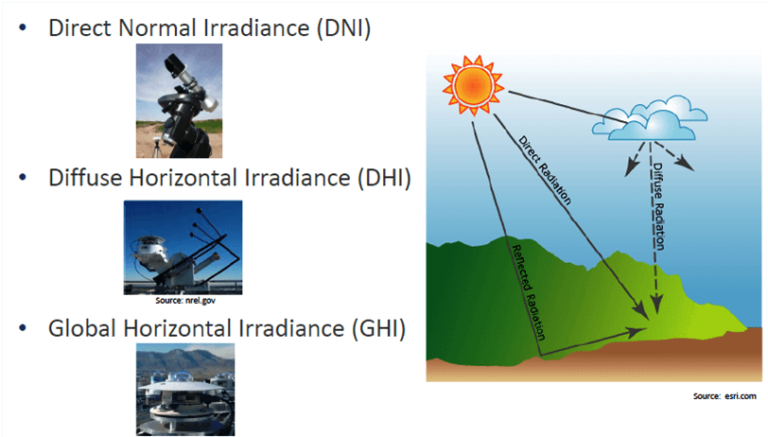
\includegraphics[width=0.7\textwidth]{./images/SoA_irrad/dni-dhi-ghi-1-768x437.png}
      \caption{Componentes de la radiación solar y los instrumentos de medida. Recuperado de \url{http://web.archive.org/web/20230624215046/https://yellowhaze.in/wp-content/uploads/2017/01/dni-dhi-ghi-1-768x437.png}}
      \label{fig:irrad_componentes}
\end{figure}

Esta radiación se descompone en tres componentes que dependen de la superficie incidente: la radiación directa, la radiación difusa y la radiación reflejada. La radiación directa es la que proviene del sol y llega directamente a la superficie de los módulos, la radiación difusa es la que proviene del cielo y se dispersa en todas direcciones, y la radiación reflejada o albedo es la que proviene de la reflexión y emisión de radiación sobre superficies cercanas. Estas componentes se suman para obtener la radiación total incidente en la superficie de los módulos, que es la que se emplea para calcular la producción de energía.

En resumen, el estado del arte de la energía solar fotovoltaica abarca una amplia gama de tecnologías, estudios y sistemas. En este Trabajo de Fin de Grado se tratarán algunas de las propuestas que se han realizado en el ámbito de la simulación y en el análisis de sistemas fotovoltaicos, con el enfoque particular en la librería \textit{pvlib-python}.

\section{Simulación de sistemas fotovoltaicos} \label{sct:simulaciones}

La importancia de simulaciones y análisis previo a la implantación de sistemas fotovoltaicos tanto para inversores, operaciones de financiación y diseñadores ha dado lugar a múltiples herramientas software y modelos como PVWatts, PVGIS, PV-Online, PV*SOL, PVsyst, System Advisor Model (SAM) y muchas más \cite{stein_models_2009, Kumar_2017}. Normalmente estas herramientas propietarias ponen el foco en calcular el rédito energético y económico de una instalación fotovoltaica, pero no en el desarrollo de la investigación y validación de modelos científicos. La Sección \ref{sct:pvlib} mostrará que la librería \textit{pvlib-python} se centra en la investigación y validación de modelos científicos para la simulación de sistemas fotovoltaicos, mientras se obvia el cálculo de coste y rédito económico.

Dentro de este grupo de herramientas, surge la iniciativa de código abierto PV\_LIB-MatLab con origen en la institución \textit{Sandia National Laboratories, EEUU}, hacia el año 2009 \cite{Stein_Holmgren_Forbess_Hansen_2016}. Posteriormente, en 2013\footnote{Véase \url{https://web.archive.org/web/20240411190506/https://pvlib-python.readthedocs.io/en/stable/\#history-and-acknowledgement}.} se inicia el desarrollo una versión traducida en Python \cite{Anderson_Hansen_Holmgren_Jensen_Mikofski_Driesse_2023, Stein_2012, Andrews_Stein_Hansen_Riley_2014, Holmgren_Andrews_Lorenzo_Stein_2015, Holmgren_Groenendyk_2016}, que es sobre la que versa este trabajo.

La librería \textit{pvlib-python} aporta una serie de mejoras entre las que destacan la infraestructura de tests, la documentación y otros procedimientos de Integración Continua y Desarrollo Continuo (\textit{CI/CD}) que facilitan el desarrollo. Además, está escrita en un lenguaje de programación libre y gratuito. Por el contrario, en PV\_LIB-MatLab no existen tests, el control de versiones resulta más confuso e inaccesible al estar en un documento de Microsoft Word y, en general, hay falta de mantenimiento\footnote{Véase \url{http://web.archive.org/web/20211207215130/https://pvlib-python.readthedocs.io/en/v0.9.0/comparison_pvlib_matlab.html}.}.

\section{La librería pvlib-python} \label{sct:pvlib}

La librería \textit{pvlib-python} es una biblioteca de código abierto que proporciona herramientas para la simulación, análisis e investigación de sistemas fotovoltaicos. Se encuentra desarrollada para el lenguaje de programación interpretado Python \cite{CS-R9526}, que es ampliamente utilizado en las comunidades científica y de desarrollo de software por su sintaxis sencilla, facilidad de desarrollo y diseño orientado a objetos.

Como todo proyecto de código abierto que se encuentra en constante desarrollo, esta librería cuenta con un grupo de desarrolladores y colaboradores que contribuyen a su mantenimiento y mejora continua. Estas personas partícipes del proyecto son mayoritariamente personal dedicado a la ciencia e investigación en diferentes instituciones y universidades públicas, aunque también existe personal de ingeniería e investigación del ámbito privado. El código y la colaboración se realiza a través del repositorio de código abierto en GitHub\footnote{Véase \url{https://github.com/pvlib/pvlib-python}.}.

El código se encuentra disponible al público bajo la licencia \textit{BSD 3-Clause}\footnote{Texto de la licencia disponible en \url{https://opensource.org/license/BSD-3-clause}.}, que permite su uso, modificación, redistribución y uso en otros proyectos siempre que haga la atribución de autoría pertinente y no emplee la imagen de \textit{pvlib-python} con fines publicitarios o promotores. La librería se distribuye a través del índice de paquetes de Python, PyPI\footnote{Véase \url{https://pypi.org/project/pvlib/}.}, y en el canal de \textit{conda-forge}\footnote{Véase \url{https://anaconda.org/conda-forge/pvlib}.} para la distribución \textit{Conda}, orientada a facilitar conjuntos de librerías para ciencia de datos de forma estable y robusta. \textit{Conda} se distribuye en dos \textit{flavours} -sabores o conjuntos de librerías- conocidas como \textit{Anaconda} y \textit{Miniconda}, cada una con sus propias características y ventajas en tiempo de instalación, espacio en disco y paquetes preinstalados.

La documentación de la librería\footnote{Accesible en \url{https://pvlib-python.readthedocs.io/en/stable/}} se encuentra disponible en la plataforma\\ \mbox{\textit{ReadTheDocs}}, donde se detallan las funcionalidades, los ejemplos de uso, la estructura del código -la API\footnote{API es la contracción de \textit{Application Programming Interface} y se trata del conjunto de utilidades del que disponen los usuarios de la librería.}-, las herramientas de desarrollo, las directrices para contribuir al proyecto y la historia de cambios y versiones. La documentación se encuentra disponible exclusivamente en inglés.

\subsection{Objetivos de la librería} \label{ssct:pvlib:objetivos}

Como se ha comentado anteriormente, la librería \textit{pvlib-python} tiene como objetivo principal proporcionar herramientas para la simulación, análisis e investigación de sistemas fotovoltaicos. Para ello, cuenta con una serie de funciones y clases que permiten realizar cálculos de radiación solar, generación de energía, sombreado, eficiencia de módulos y pérdidas de energía, entre otros. Estas herramientas se basan en modelos científicos y métodos de cálculo validados por la comunidad científica y se han implementado en Python para facilitar su uso y extensión. Es importante denotar que los autores pretenden establecer la implementación de la librería como una referencia fiable y certera de los modelos científicos que se emplean en la simulación de sistemas fotovoltaicos, poniendo un enfoque especial en la rigurosidad de las publicaciones y artículos científicos que se emplean como base.

Enumerando los objetivos de la librería, se pueden destacar los siguientes:

\begin{enumerate}
      \item Proporcionar herramientas para la simulación y análisis de sistemas fotovoltaicos.
      \item Implementar modelos científicos y métodos de cálculo validados por la comunidad científica.
      \item Establecer un referente fiable de las implementaciones de las características citadas anteriormente.
      \item Auditar las contribuciones para garantizar la funcionalidad de las aportaciones.
      \item Facilitar la integración con servicios de datos meteorológicos y bases de datos de radiación solar.
      \item Fomentar la colaboración y la contribución de la comunidad científica y de desarrollo de software.
\end{enumerate}

Cabe destacar que también hay fines que se excluyen de ser objetivos, es decir, características que no se pretenden implementar o documentar. Entre estos destacan:

\begin{enumerate}
      \item Proporcionar contenido didáctico sobre la energía solar fotovoltaica, más allá del estrictamente necesario para entender y aplicar las utilidades disponibles.
      \item Hacer inferencias, sugerencias o recomendaciones que no estén publicadas formalmente sobre el uso de los modelos implementados.
      \item Facilitar un sistema \textit{ready-to-go} para usuarios finales.
\end{enumerate}

Puede parecer que excluir estos objetivos son limitantes en cuanto a la divulgación y al alcance, pero en realidad se trata de una forma de garantizar la calidad y la fiabilidad de la librería. Así el esfuerzo limitado de los mantenedores y los contribuyentes se centra en la implementación rigurosa de publicaciones de la comunidad científica.

Una nota importante, en especial sobre el último punto, es que la definición de la misma librería es que se trata de una \textit{toolbox}\footnote{En español, ``caja de herramientas''. \url{https://github.com/pvlib/pvlib-python/blob/99619e8fc5aea5c5dc4dacabb75b617786cc4a1a/README.md?plain=1\#L61}}. Esta nota es en contraposición a las herramientas de simulación y análisis de sistemas fotovoltaicos comerciales, que limitan y simplifican la experiencia del usuario, varias veces dejando de lado la documentación y la transparencia de los cálculos\footnote{Como hecho anecdótico, se puede observar alguna crítica sobre esto entre los partícipes del proyecto, por ejemplo en \url{https://github.com/pvlib/pvlib-python/issues/2057\#issuecomment-2197279047}.}.

\subsection{Funcionalidades} \label{ssct:pvlib:funcionalidades}

El proyecto de código abierto \textit{pvlib-python} cuenta múltiples características que abarcan un amplio rango de temas relacionados con la producción de energía solar fotovoltaica. Al momento de la redacción de este documento, la versión de la librería es la 0.11.0, publicada el 21 de junio de 2024. A continuación, se detallan algunas de las funcionalidades más destacadas:

\begin{itemize}
      \item Cálculo de la posición del sol: para determinar la posición del sol en el cielo en función de la localización y la hora del día, en el submódulo \texttt{pvlib.solarposition}.
      \item Cálculo de valores estándares de la radiación solar: la librería proporciona herramientas para calcular la radiación solar en una superficie plana y horizontal en función de la localización, la posición del sol y parámetros atmosféricos. Véase \texttt{pvlib.solarposition} y \texttt{pvlib.clearsky}.
      \item Procedimientos de descomposición, transposición y transposición inversa de la radiación solar: se emplean para, a partir de la irradiance solar en una superficie plana y horizontal, obtener la incidente en un colector plano orientado arbitrariamente. Y una vez obtenidas las componentes directa, difusa y de albedo de esta irradiancia, aplicar correcciones convenientes para obtener la radiación efectiva colectada en la superficie. También se puede realizar el proceso inverso, de las componentes en el plano inclinado a la radiación en una superficie plana y horizontal. Estas utilidades se encuentran en el submódulo \texttt{pvlib.irradiance}.
      \item Obtención de parámetros atmosféricos como la columna o masa de aire, un número que representa cuánta atmósfera hay, relativa a la columna completamente vertical (\texttt{AM=1}), en el submódulo \texttt{pvlib.atmosphere}.
      \item Valores de albedo predefinidos, bien de materiales sólidos o de superficies naturales de agua, en \texttt{pvlib.albedo}.
      \item Corrección de la radiación incidente en función del ángulo de incidencia: debido a la reflexión que sufre la luz solar al incidir en una superficie de forma oblicua. Las utilidades se encuentran en el submódulo \texttt{pvlib.iam}.
      \item Producción fotovoltaica: mediante puntos característicos como el de máxima potencia (\textit{MPP}) o calculando curvas I-V completas. Se emplean modelos de eficiencia de módulos y pérdidas de energía para estimar la producción de energía en un sistema fotovoltaico, mediante el modelo de un único diodo. Se encuentra en el submódulo \texttt{pvlib.singlediode}.
      \item Cálculo de sombreado: métodos analíticos para calcular la fracción sombreada de hileras de filas. Véase el submódulo \texttt{pvlib.shading}.
      \item Cálculo de ángulos de seguimiento: para seguidores de uno y dos ejes, que permitan colectar la máxima radiación solar directa, que normalmente se corresponderá con la máxima producción de energía. Véase el submódulo \texttt{pvlib.tracking}.
      \item Cálculo de temperatura de los módulos: normalmente empíricos, facilitan estimar la producción de energía ya que, habitualmente, la eficiencia de las células es bastante susceptible a la temperatura. Estas utilidades se encuentran en \texttt{pvlib.temperature}.
      \item Estimación de ganancias o pérdidas por efectos del espectro solar: pues en función de la composición del espectro solar incidente en los módulos, la eficiencia de los mismos puede variar. En \texttt{pvlib.spectrum}.
      \item Modelado de eficiencia de inversores: para estimar la eficiencia de los inversores DC-AC en función de la potencia de entrada y sus demás características. En \texttt{pvlib.inverter}.
      \item Modelado de pérdidas en transformadores: para estimar las pérdidas en los transformadores de conexión a red. En \texttt{pvlib.transformer}.
      \item Modelado de pérdidas en cables: para estimar las pérdidas resistivas en los cables. En \texttt{pvlib.pvsystem}.
      \item Integración de APIs externas para la obtención de datos meteorológicos relacionados con la fotovoltaica, en \texttt{pvlib.iotools}.
      \item Abstracciones de los componentes que conforman una instalación fotovoltaica, mediante las clases \texttt{Location}, \texttt{Array}, \texttt{PVSystem} y la clase que agrupa el flujo computacional \texttt{Modelchain}, en los submódulos \texttt{pvlib.location}, \texttt{pvlib.pvsystem} y \texttt{pvlib.modelchain}.
      \item Cálculos adicionales para sistemas bifaciales, que son aquellos colectores planos que permiten la captación de radiación solar por ambas caras del módulo. En \texttt{pvlib.bifacial}.

\end{itemize}

\subsection{Repositorio del proyecto} \label{ssct:pvlib:repositorio}

Como se ha mencionado anteriormente, el código de la librería \textit{pvlib-python} se encuentra alojado en un repositorio de código abierto. Un repositorio es una carpeta que contiene una series de archivos, de los cuales los más importantes se gestionan mediante un sistema de control de versiones, \textit{VCS} por sus siglas en inglés. Este sistema permite llevar un registro de los cambios realizados en los archivos, así como la posibilidad de volver a versiones anteriores en caso de que se produzca un error o un fallo en el código. El uso de esta herramienta es indispensable en proyectos de software, ya que facilita la colaboración entre los desarrolladores y la gestión de las versiones del código.

En el caso de \textit{pvlib-python}, el repositorio se encuentra alojado en la plataforma GitHub, que es una de las más populares para el alojamiento de proyectos de código abierto.

El repositorio cuenta con múltiples archivos y sub-carpetas que configuran el proyecto. Algunos de los más destacables son:

\begin{itemize}
      \item \texttt{README.md}: es el primer archivo en verse en la plataforma online y contiene la descripción del proyecto, su propósito y cómo instalarlo, entre otros.
      \item \texttt{LICENSE}: es el archivo que contiene la licencia del proyecto, en este caso la licencia \textit{BSD 3-Clause}.
      \item \texttt{pyproject.toml}, \texttt{setup.cfg}, \texttt{setup.py}, \texttt{MANIFEST.in}: son los archivos que definen la configuración del proyecto, como el nombre, la versión, la descripción, las dependencias, los archivos que componen una distribución precompilada o de código fuente, etc. que las personas usuarias verán en la plataformas de distribución de paquetes.
      \item \texttt{docs/}: es la carpeta que contiene archivos de configuración y explicativos que permiten generar la documentación del proyecto. No obstante, el código que se expone públicamente se documenta automáticamente a partir de unos comentarios en el código.
      \item \texttt{pvlib/}: es la carpeta que contiene el código fuente de la librería, organizado en sub-carpetas y archivos según su funcionalidad. Los tests unitarios y de integración se encuentran en esta carpeta.
      \item \texttt{AUTHORS.md}, \texttt{CODE\_OF\_CONDUCT.md}, \texttt{codecov.yml}, \texttt{readthedocs.yml}, \texttt{paper/}, \texttt{ci/}, \texttt{benchmarks/} y \texttt{.github/}: son archivos y carpetas que contienen información adicional sobre el proyecto y la configuración de todos los flujos de integración continua: destacan los tests, los benchmarks y la documentación.

\end{itemize}

\subsection{Frameworks de desarrollo del proyecto} \label{sct:pvlib:dev}

Como tal, el desarrollo del proyecto requiere el conocimiento de algunas herramientas que permiten la colaboración con el repositorio principal y cumplir con las directrices para contribuir al proyecto. Estas se suelen denominar \textit{frameworks} de desarrollo, literalmente marcos de trabajo, que normalizan la forma de desarrollar y colaborar en el proyecto.

La elección de las herramientas empleadas corresponde a una preferencia en cuanto a uso y extensión en el desarrollo software, pero pueden variar en el futuro, como ya lo ha hecho en el pasado.

En el lado de las utilidades esenciales, se encuentran:

\begin{itemize}
      \item \textit{Git}: como sistema de control de versiones que se emplea para gestionar los cambios en el código.
      \item \textit{GitHub}: es la plataforma de alojamiento de proyectos de código abierto que se emplea para colaborar en el desarrollo del proyecto. Permite crear \textit{issues} o discusiones para reportar errores o sugerir mejoras; y proponer cambios y revisarlos públicamente en \textit{pull requests}. Además proporciona máquinas virtuales para ejecutar los procedimientos de integración y desarrollo continuos.
      \item \textit{ReadTheDocs} junto con \textit{sphinx}: es la plataforma que se emplea para ejecutar \textit{sphinx}, el entorno de trabajo que produce la documentación en formato HTML, y alojar el producto. La documentación se escribe en formato \textit{reStructuredText} y se genera automáticamente a partir de los comentarios en el código, scripts con los ejemplos y archivos fuente con el cuerpo más general.
      \item \textit{pytest}: es la librería de Python que se emplea para escribir y ejecutar tests unitarios y de integración en el código. Facilita la creación de \textit{mocks} u observadores del estado de partes del mismo proyecto, la reutilización de datos de tests, la ejecución opcional de los tests en función de las dependencias disponibles y visualizar los resultados en un informe. Posiblemente la mejor característica es poder ejecutar los tests uno a uno, por grupo o todos a la vez.
      \item \textit{Codecov}: es la plataforma que se emplea para medir la cobertura de los tests en el código. Permite visualizar la cobertura de los tests en un informe y comprobar si se están realizando pruebas suficientes en el código.
      \item \textit{flake8}: es una utilidad que detecta errores de estilo en el código, como la longitud de las líneas, la indentación, la presencia de espacios en blanco, entre otros. Facilita la escritura de código limpio y legible, por ende, mantenible.
      Además, facilita la detección de errores estáticos en el código; esto es, condicionales que nunca se cumplen, variables que no se usan, importación innecesaria de módulos, identificadores duplicadas o que no siguen la convención de nombres, entre otros.

\end{itemize}

